% Options for packages loaded elsewhere
\PassOptionsToPackage{unicode}{hyperref}
\PassOptionsToPackage{hyphens}{url}
%
\documentclass[
  letterpaper,
  paper=6in:9in,
  pagesize=pdftex,
  headinclude=on,
  footinclude=on,
  12pt]{scrbook}

\usepackage{amsmath,amssymb}
\usepackage{iftex}
\ifPDFTeX
  \usepackage[T1]{fontenc}
  \usepackage[utf8]{inputenc}
  \usepackage{textcomp} % provide euro and other symbols
\else % if luatex or xetex
  \usepackage{unicode-math}
  \defaultfontfeatures{Scale=MatchLowercase}
  \defaultfontfeatures[\rmfamily]{Ligatures=TeX,Scale=1}
\fi
\usepackage{lmodern}
\ifPDFTeX\else  
    % xetex/luatex font selection
\fi
% Use upquote if available, for straight quotes in verbatim environments
\IfFileExists{upquote.sty}{\usepackage{upquote}}{}
\IfFileExists{microtype.sty}{% use microtype if available
  \usepackage[]{microtype}
  \UseMicrotypeSet[protrusion]{basicmath} % disable protrusion for tt fonts
}{}
\makeatletter
\@ifundefined{KOMAClassName}{% if non-KOMA class
  \IfFileExists{parskip.sty}{%
    \usepackage{parskip}
  }{% else
    \setlength{\parindent}{0pt}
    \setlength{\parskip}{6pt plus 2pt minus 1pt}}
}{% if KOMA class
  \KOMAoptions{parskip=half}}
\makeatother
\usepackage{xcolor}
\setlength{\emergencystretch}{3em} % prevent overfull lines
\setcounter{secnumdepth}{5}
% Make \paragraph and \subparagraph free-standing
\ifx\paragraph\undefined\else
  \let\oldparagraph\paragraph
  \renewcommand{\paragraph}[1]{\oldparagraph{#1}\mbox{}}
\fi
\ifx\subparagraph\undefined\else
  \let\oldsubparagraph\subparagraph
  \renewcommand{\subparagraph}[1]{\oldsubparagraph{#1}\mbox{}}
\fi

\usepackage{color}
\usepackage{fancyvrb}
\newcommand{\VerbBar}{|}
\newcommand{\VERB}{\Verb[commandchars=\\\{\}]}
\DefineVerbatimEnvironment{Highlighting}{Verbatim}{commandchars=\\\{\}}
% Add ',fontsize=\small' for more characters per line
\usepackage{framed}
\definecolor{shadecolor}{RGB}{241,243,245}
\newenvironment{Shaded}{\begin{snugshade}}{\end{snugshade}}
\newcommand{\AlertTok}[1]{\textcolor[rgb]{0.68,0.00,0.00}{#1}}
\newcommand{\AnnotationTok}[1]{\textcolor[rgb]{0.37,0.37,0.37}{#1}}
\newcommand{\AttributeTok}[1]{\textcolor[rgb]{0.40,0.45,0.13}{#1}}
\newcommand{\BaseNTok}[1]{\textcolor[rgb]{0.68,0.00,0.00}{#1}}
\newcommand{\BuiltInTok}[1]{\textcolor[rgb]{0.00,0.23,0.31}{#1}}
\newcommand{\CharTok}[1]{\textcolor[rgb]{0.13,0.47,0.30}{#1}}
\newcommand{\CommentTok}[1]{\textcolor[rgb]{0.37,0.37,0.37}{#1}}
\newcommand{\CommentVarTok}[1]{\textcolor[rgb]{0.37,0.37,0.37}{\textit{#1}}}
\newcommand{\ConstantTok}[1]{\textcolor[rgb]{0.56,0.35,0.01}{#1}}
\newcommand{\ControlFlowTok}[1]{\textcolor[rgb]{0.00,0.23,0.31}{#1}}
\newcommand{\DataTypeTok}[1]{\textcolor[rgb]{0.68,0.00,0.00}{#1}}
\newcommand{\DecValTok}[1]{\textcolor[rgb]{0.68,0.00,0.00}{#1}}
\newcommand{\DocumentationTok}[1]{\textcolor[rgb]{0.37,0.37,0.37}{\textit{#1}}}
\newcommand{\ErrorTok}[1]{\textcolor[rgb]{0.68,0.00,0.00}{#1}}
\newcommand{\ExtensionTok}[1]{\textcolor[rgb]{0.00,0.23,0.31}{#1}}
\newcommand{\FloatTok}[1]{\textcolor[rgb]{0.68,0.00,0.00}{#1}}
\newcommand{\FunctionTok}[1]{\textcolor[rgb]{0.28,0.35,0.67}{#1}}
\newcommand{\ImportTok}[1]{\textcolor[rgb]{0.00,0.46,0.62}{#1}}
\newcommand{\InformationTok}[1]{\textcolor[rgb]{0.37,0.37,0.37}{#1}}
\newcommand{\KeywordTok}[1]{\textcolor[rgb]{0.00,0.23,0.31}{#1}}
\newcommand{\NormalTok}[1]{\textcolor[rgb]{0.00,0.23,0.31}{#1}}
\newcommand{\OperatorTok}[1]{\textcolor[rgb]{0.37,0.37,0.37}{#1}}
\newcommand{\OtherTok}[1]{\textcolor[rgb]{0.00,0.23,0.31}{#1}}
\newcommand{\PreprocessorTok}[1]{\textcolor[rgb]{0.68,0.00,0.00}{#1}}
\newcommand{\RegionMarkerTok}[1]{\textcolor[rgb]{0.00,0.23,0.31}{#1}}
\newcommand{\SpecialCharTok}[1]{\textcolor[rgb]{0.37,0.37,0.37}{#1}}
\newcommand{\SpecialStringTok}[1]{\textcolor[rgb]{0.13,0.47,0.30}{#1}}
\newcommand{\StringTok}[1]{\textcolor[rgb]{0.13,0.47,0.30}{#1}}
\newcommand{\VariableTok}[1]{\textcolor[rgb]{0.07,0.07,0.07}{#1}}
\newcommand{\VerbatimStringTok}[1]{\textcolor[rgb]{0.13,0.47,0.30}{#1}}
\newcommand{\WarningTok}[1]{\textcolor[rgb]{0.37,0.37,0.37}{\textit{#1}}}

\providecommand{\tightlist}{%
  \setlength{\itemsep}{0pt}\setlength{\parskip}{0pt}}\usepackage{longtable,booktabs,array}
\usepackage{calc} % for calculating minipage widths
% Correct order of tables after \paragraph or \subparagraph
\usepackage{etoolbox}
\makeatletter
\patchcmd\longtable{\par}{\if@noskipsec\mbox{}\fi\par}{}{}
\makeatother
% Allow footnotes in longtable head/foot
\IfFileExists{footnotehyper.sty}{\usepackage{footnotehyper}}{\usepackage{footnote}}
\makesavenoteenv{longtable}
\usepackage{graphicx}
\makeatletter
\def\maxwidth{\ifdim\Gin@nat@width>\linewidth\linewidth\else\Gin@nat@width\fi}
\def\maxheight{\ifdim\Gin@nat@height>\textheight\textheight\else\Gin@nat@height\fi}
\makeatother
% Scale images if necessary, so that they will not overflow the page
% margins by default, and it is still possible to overwrite the defaults
% using explicit options in \includegraphics[width, height, ...]{}
\setkeys{Gin}{width=\maxwidth,height=\maxheight,keepaspectratio}
% Set default figure placement to htbp
\makeatletter
\def\fps@figure{htbp}
\makeatother

\usepackage{fvextra}
\DefineVerbatimEnvironment{Highlighting}{Verbatim}{breaklines,commandchars=\\\{\}}
\areaset[0.50in]{4.5in}{8in}
\makeatletter
\makeatother
\makeatletter
\@ifpackageloaded{bookmark}{}{\usepackage{bookmark}}
\makeatother
\makeatletter
\@ifpackageloaded{caption}{}{\usepackage{caption}}
\AtBeginDocument{%
\ifdefined\contentsname
  \renewcommand*\contentsname{Table of contents}
\else
  \newcommand\contentsname{Table of contents}
\fi
\ifdefined\listfigurename
  \renewcommand*\listfigurename{List of Figures}
\else
  \newcommand\listfigurename{List of Figures}
\fi
\ifdefined\listtablename
  \renewcommand*\listtablename{List of Tables}
\else
  \newcommand\listtablename{List of Tables}
\fi
\ifdefined\figurename
  \renewcommand*\figurename{Figure}
\else
  \newcommand\figurename{Figure}
\fi
\ifdefined\tablename
  \renewcommand*\tablename{Table}
\else
  \newcommand\tablename{Table}
\fi
}
\@ifpackageloaded{float}{}{\usepackage{float}}
\floatstyle{ruled}
\@ifundefined{c@chapter}{\newfloat{codelisting}{h}{lop}}{\newfloat{codelisting}{h}{lop}[chapter]}
\floatname{codelisting}{Listing}
\newcommand*\listoflistings{\listof{codelisting}{List of Listings}}
\makeatother
\makeatletter
\@ifpackageloaded{caption}{}{\usepackage{caption}}
\@ifpackageloaded{subcaption}{}{\usepackage{subcaption}}
\makeatother
\makeatletter
\@ifpackageloaded{tcolorbox}{}{\usepackage[skins,breakable]{tcolorbox}}
\makeatother
\makeatletter
\@ifundefined{shadecolor}{\definecolor{shadecolor}{rgb}{.97, .97, .97}}
\makeatother
\makeatletter
\makeatother
\makeatletter
\makeatother
\ifLuaTeX
  \usepackage{selnolig}  % disable illegal ligatures
\fi
\IfFileExists{bookmark.sty}{\usepackage{bookmark}}{\usepackage{hyperref}}
\IfFileExists{xurl.sty}{\usepackage{xurl}}{} % add URL line breaks if available
\urlstyle{same} % disable monospaced font for URLs
\hypersetup{
  pdftitle={ChatGPT com R},
  pdfauthor={Bruno A Lima},
  hidelinks,
  pdfcreator={LaTeX via pandoc}}

\title{ChatGPT com R}
\author{Bruno A Lima}
\date{2023-10-29}

\begin{document}
\frontmatter
\maketitle
\RecustomVerbatimEnvironment{verbatim}{Verbatim}{
   showspaces = false,
   showtabs = false,
   breaksymbolleft={},
   breaklines
   % Note: setting commandchars=\\\{\} here will cause an error
}

\ifdefined\Shaded\renewenvironment{Shaded}{\begin{tcolorbox}[enhanced, frame hidden, breakable, boxrule=0pt, interior hidden, borderline west={3pt}{0pt}{shadecolor}, sharp corners]}{\end{tcolorbox}}\fi

\renewcommand*\contentsname{Table of contents}
{
\setcounter{tocdepth}{2}
\tableofcontents
}
\mainmatter
\bookmarksetup{startatroot}

\hypertarget{um-simples-tutorial}{%
\chapter*{Um simples tutorial}\label{um-simples-tutorial}}
\addcontentsline{toc}{chapter}{Um simples tutorial}

\markboth{Um simples tutorial}{Um simples tutorial}

\begin{figure}[H]

{\centering 
\includegraphics{images/chatgpt_r.jpg}

}

\caption{\label{fig-gosling}chatGPT through RStudio}

\end{figure}

Livro de instruções para usar o \emph{chatGPT} com a linguagem \emph{R}.

\bookmarksetup{startatroot}

\hypertarget{prefuxe1cio}{%
\chapter{Prefácio}\label{prefuxe1cio}}

Este tutorial tem por base o MOOC
\href{https://learn.deeplearning.ai/}{ChatGPT Prompt Engineering for
Developers}.

As instruções que naquele \emph{short course} são apresentadas com
exemplos em \emph{python}, aqui são replicadas com recurso à linguagem
\textbf{R}.

O \emph{package}
\href{https://cloud.r-project.org/web/packages/openai/index.html}{\{openai\}}
é usado para o R aceder à API do chatGPT e obter as respontas
pretendidas.

Antes de mais temos de definir a nossa chave API dada pelo OpenAI tal
como descrito no sitio do
\href{https://irudnyts.github.io/openai/}{openai}:

\begin{Shaded}
\begin{Highlighting}[]
\FunctionTok{Sys.setenv}\NormalTok{(}
    \AttributeTok{OPENAI\_API\_KEY =} \StringTok{\textquotesingle{}sk{-}xxxxxxxxxxxxxxxxxxxxxxxxxxxxxxxxxxxxxxxxxxxxxxxx\textquotesingle{}}
\NormalTok{)}
\end{Highlighting}
\end{Shaded}

Podemos deferir dois tipos de de \emph{Large Language Models} (LLM):

\begin{itemize}
\item
  Base LLM - prevê a próxima palavra, tem por base texto como dados de
  treino;
\item
  Instruction Tuned LLM - Tenta seguir instruções, \emph{fine-tune} com
  instruções e em tentativas bem sucedidas no seguimento dessas
  instruções. \emph{Reinforcement Learning with Human Feedback} (RLHF)
\end{itemize}

\bookmarksetup{startatroot}

\hypertarget{guidelines}{%
\chapter{Guidelines}\label{guidelines}}

Com o \emph{package} \{openai\}, começamos por definir uma função de
ajuda para usar \emph{prompts} e gerar \emph{outputs}. Nestes exemplos
usaremos o modelo \texttt{gpt-3.5-turbo} do OpenAI e o
\href{https://platform.openai.com/docs/guides/chat}{chat completions
endpoint.}.

\begin{Shaded}
\begin{Highlighting}[]
\FunctionTok{library}\NormalTok{(openai)}

\NormalTok{get\_completion }\OtherTok{\textless{}{-}} \ControlFlowTok{function}\NormalTok{(prompt, }\AttributeTok{model =} \StringTok{"gpt{-}3.5{-}turbo"}\NormalTok{, ...)\{}
\NormalTok{  res }\OtherTok{\textless{}{-}} \FunctionTok{create\_chat\_completion}\NormalTok{(}
    \AttributeTok{model =}\NormalTok{ model,}
    \AttributeTok{messages =} \FunctionTok{list}\NormalTok{(}
      \FunctionTok{list}\NormalTok{(}
        \StringTok{"role"} \OtherTok{=} \StringTok{"user"}\NormalTok{,}
        \StringTok{"content"} \OtherTok{=}\NormalTok{ prompt}
\NormalTok{      )}
\NormalTok{    ), ...}
\NormalTok{  )}

  \FunctionTok{return}\NormalTok{(res}\SpecialCharTok{$}\NormalTok{choices}\SpecialCharTok{$}\NormalTok{message.content)}
\NormalTok{\}}
\end{Highlighting}
\end{Shaded}

\hypertarget{princuxedpios-para-prompting}{%
\section{\texorpdfstring{Princípios para
\emph{prompting}}{Princípios para prompting}}\label{princuxedpios-para-prompting}}

\begin{enumerate}
\def\labelenumi{\arabic{enumi}.}
\tightlist
\item
  Escrever instruções claras e específicas;
\item
  Dar tempo ao modelo para pensar.
\end{enumerate}

\hypertarget{escrever-instruuxe7uxf5es-claras-e-especuxedficas}{%
\subsection{Escrever instruções claras e
específicas;}\label{escrever-instruuxe7uxf5es-claras-e-especuxedficas}}

\hypertarget{tuxe1tica-1}{%
\subsubsection{Tática 1:}\label{tuxe1tica-1}}

Usar delimitadores para distinguir de forma clara diferentes partes do
\emph{input}:

\begin{itemize}
\tightlist
\item
  delimitadores como: ```, ``\,``, ---, \textless{} \textgreater, , :
\end{itemize}

\begin{Shaded}
\begin{Highlighting}[]
\NormalTok{texto }\OtherTok{\textless{}{-}} \StringTok{"Devemos expressar com instruções claras e específicas o que pretendemos do modelo. }
\StringTok{Isto guiará o modelo para o output desejado e reduzirá as probabilidade de }
\StringTok{receber respostas incorrectas ou irrelevante. Muitas vezes, }
\StringTok{prompts mais largos providenciam um contexto para o modelo o que pode gerar outputs mais relevantes e detalhados"}

\NormalTok{prompt0 }\OtherTok{\textless{}{-}} \FunctionTok{paste}\NormalTok{(}\StringTok{\textquotesingle{}Resume o texto delimitado por acentos triplos numa única frase curta: }
\StringTok{                 \textasciigrave{}\textasciigrave{}\textasciigrave{}\textquotesingle{}}\NormalTok{, texto, }\StringTok{\textquotesingle{}\textasciigrave{}\textasciigrave{}\textquotesingle{}}\NormalTok{)}

\NormalTok{resposta }\OtherTok{\textless{}{-}} \FunctionTok{get\_completion}\NormalTok{(prompt0)}

\NormalTok{resposta}
\end{Highlighting}
\end{Shaded}

O uso de delimitadores é também uma forma de garantir que um terceiro
utilizador não dá instruções que condicionem um determinado tipo de
resposta que queremos obter. Assim, também é possível fazer funções
auxiliares com um \emph{prompt} pré-definido.

\hypertarget{tuxe1ctica-2}{%
\subsubsection{Táctica 2:}\label{tuxe1ctica-2}}

Pedir um \emph{oputput} estruturado

\begin{itemize}
\tightlist
\item
  JSON, HTML
\end{itemize}

\begin{Shaded}
\begin{Highlighting}[]
\NormalTok{prompt1 }\OtherTok{\textless{}{-}} \StringTok{"Gera uma lista de três livros inventados com os seus autores e géneros respectivos. }
\StringTok{Devolve um JSON com as seguintes chaves: book\_id, title, author, genre"} 

\NormalTok{resposta }\OtherTok{\textless{}{-}} \FunctionTok{get\_completion}\NormalTok{(prompt1)}

\NormalTok{resposta}
\end{Highlighting}
\end{Shaded}

\hypertarget{tuxe1ctica-3}{%
\subsubsection{Táctica 3:}\label{tuxe1ctica-3}}

Pedir ao modelo para \emph{checkar} se as condições foram satisfeitas.

\begin{Shaded}
\begin{Highlighting}[]
\NormalTok{texto\_2 }\OtherTok{\textless{}{-}} \StringTok{"fazer uma taça de chá é fácil! Primeiro precisamos de por água a ferver. }
\StringTok{Enquanto isto acontece, pegamos numa taça e colocamos uma saqueta de chá. }
\StringTok{Quando a água estiver quente vertemos sobre a saqueta de chá. }
\StringTok{Depois de ums minutos podemos retirar a saqueta. Se quisermos, }
\StringTok{podemos adicionar açucar ou leite para lhe dar mais sabor. E é só. }
\StringTok{Podemos agora desfrutar de um delicioso chá."}

\NormalTok{prompt2 }\OtherTok{\textless{}{-}} \FunctionTok{paste}\NormalTok{(}\StringTok{"Vou dar{-}te um texto delimitado por triplas pelicas. }
\StringTok{Se tiver uma sequencia de instruções, re{-}escreve essas ionstruções no seguinte formato:}
\StringTok{                 passo 1 {-} ...}
\StringTok{                 passo 2 {-} ...}
\StringTok{                 ...}
\StringTok{                 passo n {-} ...}
\StringTok{                 Se o texto não tiver uma sequência de instruçõpes então escreve }
\StringTok{\textquotesingle{}Não há passos a seguir!\textquotesingle{}}
\StringTok{\textquotesingle{}\textquotesingle{}\textquotesingle{} "}\NormalTok{, texto\_2, }\StringTok{"\textquotesingle{}\textquotesingle{}\textquotesingle{}"}\NormalTok{)}

\NormalTok{resposta }\OtherTok{\textless{}{-}} \FunctionTok{get\_completion}\NormalTok{(prompt2)}

\NormalTok{resposta}
\end{Highlighting}
\end{Shaded}

\begin{Shaded}
\begin{Highlighting}[]
\NormalTok{texto\_3 }\OtherTok{\textless{}{-}} \StringTok{"Hoje, o sol brilha e os pássaros cantam. Está um bonito dia para passear no parque. }
\StringTok{As flores rebentam e as arvores balanceiam com o vento. As pessoas disfrutam do bom tempo."}

\NormalTok{prompt3 }\OtherTok{\textless{}{-}} \FunctionTok{paste}\NormalTok{(}\StringTok{"Vou dar{-}te um texto delimitado por triplas pelicas. Se tiver uma sequencia de instruções, re{-}escreve essas ionstruções no seguinte formato:}
\StringTok{                 passo 1 {-} ...}
\StringTok{                 passo 2 {-} ...}
\StringTok{                 ...}
\StringTok{                 passo n {-} ...}
\StringTok{                 Se o texto não tiver uma sequ{-}\textasciitilde{}encia de instruçõpes então escreve \textquotesingle{}Não há passos a seguir!\textquotesingle{}}
\StringTok{                 \textquotesingle{}\textquotesingle{}\textquotesingle{} "}\NormalTok{, texto\_3, }\StringTok{"\textquotesingle{}\textquotesingle{}\textquotesingle{}"}\NormalTok{)}

\NormalTok{resposta }\OtherTok{\textless{}{-}} \FunctionTok{get\_completion}\NormalTok{(prompt3)}

\NormalTok{resposta}
\end{Highlighting}
\end{Shaded}

\hypertarget{tuxe1ctica-4}{%
\subsubsection{Táctica 4:}\label{tuxe1ctica-4}}

Frases curtas

\begin{Shaded}
\begin{Highlighting}[]
\NormalTok{prompt4 }\OtherTok{\textless{}{-}} \StringTok{"Deves responder de forma consistente com o estilo:}
\StringTok{\textless{}criança\textgreater{}: Ensina{-}me sobre paciência.}
\StringTok{\textless{}avô\textgreater{}: O rio que escava o vale mais fundo começa numa modesta nascente; }
\StringTok{a maior sinfonia começa numa única nota; o tapete mais intrincado começa só com um fio.}
\StringTok{\textless{}criança\textgreater{}: Ensina{-}me sobre resistência."}

\NormalTok{resposta }\OtherTok{\textless{}{-}} \FunctionTok{get\_completion}\NormalTok{(prompt4)}

\NormalTok{resposta}
\end{Highlighting}
\end{Shaded}

\hypertarget{dar-tempo-ao-modelo-para-pensar}{%
\subsection{Dar tempo ao modelo para
pensar;}\label{dar-tempo-ao-modelo-para-pensar}}

\hypertarget{tuxe1tica-1-1}{%
\subsubsection{Tática 1:}\label{tuxe1tica-1-1}}

Especificar os passos necessários para completar a tarefa.

\begin{Shaded}
\begin{Highlighting}[]
\NormalTok{texto\_4 }\OtherTok{\textless{}{-}} \StringTok{"Numa charmosa aldeia, os irmãos João e José tinham a tarefe de recolher }
\StringTok{água duma poço numa colina. Enquanto subima, cantando com alegria, a má sorte atinguiu João }
\StringTok{que tropeçou numa pedra e cai colina abaixo seguido pelo José. }
\StringTok{Embora combalidos regressaram a casa para braços reconfortantes. }
\StringTok{Apesar do precalço os seus espiritos aventurosos permaneceram intactos e eles continuaram a explorar com gosto."}

\NormalTok{prompt5 }\OtherTok{\textless{}{-}} \FunctionTok{paste}\NormalTok{(}\StringTok{"completa a seguinte tarefa:}
\StringTok{                 1 {-} resume o texto que está entre plicas triplas numa só frase;}
\StringTok{                 2 {-} traduz o resumo para francês;}
\StringTok{                 3 {-} lista cada nome do resumo em francês;}
\StringTok{                 4 {-} devolve um objacto JSON com as chaves: french\_summary, num\_names.}
\StringTok{                 separa cada resposta com um paragrafo. \textquotesingle{}\textquotesingle{}\textquotesingle{} "}\NormalTok{, texto\_4, }\StringTok{"\textquotesingle{}\textquotesingle{}\textquotesingle{} "}\NormalTok{)}

\NormalTok{resposta }\OtherTok{\textless{}{-}} \FunctionTok{get\_completion}\NormalTok{(prompt5)}

\NormalTok{resposta}
\end{Highlighting}
\end{Shaded}

Pedir o output num formato específico.

\begin{Shaded}
\begin{Highlighting}[]
\NormalTok{prompt6 }\OtherTok{\textless{}{-}} \FunctionTok{paste}\NormalTok{(}\StringTok{"A tuas tarefas são:}
\StringTok{                1 {-} resume o texto entre plicas triplas, numa frase,}
\StringTok{                2 {-} traduz o resumo para francês;}
\StringTok{                3 {-} lista cada nome do resumo em francês;}
\StringTok{                4 {-} devolve um objacto JSON com as chaves: french\_summary, num\_names.}
\StringTok{                Usa o seguinte formato:}
\StringTok{Text: \textless{}texto a resumir\textgreater{}}
\StringTok{Summary: \textless{}resumo\textgreater{}}
\StringTok{Translation: \textless{}resumo traduzido\textgreater{}}
\StringTok{Names: \textless{}lista de nomes do resumo em francês\textgreater{}}
\StringTok{Output JSON: \textless{}json com resumo e nomes\textgreater{}}

\StringTok{texto: \textquotesingle{}\textquotesingle{}\textquotesingle{} "}\NormalTok{, texto\_4, }\StringTok{"\textquotesingle{}\textquotesingle{}\textquotesingle{} "}\NormalTok{)}

\NormalTok{resposta }\OtherTok{\textless{}{-}} \FunctionTok{get\_completion}\NormalTok{(prompt6)}

\NormalTok{resposta}
\end{Highlighting}
\end{Shaded}

\hypertarget{tuxe1tica-2}{%
\subsubsection{Tática 2:}\label{tuxe1tica-2}}

Instruir o modelo a trabalhar a sua própria solução antes de se
precipitar numa conclusão.

\begin{Shaded}
\begin{Highlighting}[]
\NormalTok{prompt7 }\OtherTok{\textless{}{-}} \StringTok{"Determina se a solução do aluno é correcta.}
\StringTok{questão: estou a construir uma instalação de energia solar e preciso ajuda na parte financeira.}
\StringTok{{-} preço do terreno 100€ / metro quadrado}
\StringTok{{-} paineis solares a 250€ / metro quadrado}
\StringTok{{-} contrato de manutenção que custa 100k € e mais 10€ / metro quadrado}
\StringTok{Qual é o custo total para o primeiro ano em produção em função do metro quadrado?}
\StringTok{solução do aluno: Seja x o tamanho da instalação em metros quadrados:}
\StringTok{1. custo do terreno: 100x}
\StringTok{2. custo do painel solar: 250x}
\StringTok{3. custo da manutenção: 100000 + 100x}
\StringTok{custo total: 100x + 250x + 100000 + 100x = 450x + 100000"}

\NormalTok{resposta }\OtherTok{\textless{}{-}} \FunctionTok{get\_completion}\NormalTok{(prompt7)}

\NormalTok{resposta}
\end{Highlighting}
\end{Shaded}

De notar que a resposta do aluno não é correcta.

Podemos corrigir isto, instruindo o modelo para primeiro arranjar uma
solução.

\begin{Shaded}
\begin{Highlighting}[]
\NormalTok{prompt8 }\OtherTok{\textless{}{-}} \StringTok{"A tua tarefa é determinar se a solução do aluno é correcta.}
\StringTok{Para resdolver o problema segue os passos:}
\StringTok{{-} primeiro, arranja a tua própria solução para o problema;}
\StringTok{{-} depois, compara a tua solução com a solução do aluno e avalia se a solução do aluno é correcta. }
\StringTok{Não decidas se a solução do aluno é correcta antes de tu resolveres o problema.}
\StringTok{Usa o seguinte formato:}
\StringTok{Questão:}
\StringTok{\textless{} aqui a questão \textgreater{}}
\StringTok{Solução do aluno:}
\StringTok{\textless{} aqui a solução do aluno \textgreater{}}
\StringTok{Solução correcta:}
\StringTok{\textless{} aqui a solução correta e os passos usados para chegar a esta solução \textgreater{}}
\StringTok{Nota do aluno:}
\StringTok{\textless{} correcto ou incorrecto \textgreater{}}

\StringTok{Questão:}
\StringTok{\textless{} estou a construir uma instalação de energia solar e preciso ajuda na parte financeira.}
\StringTok{{-} preço do terreno 100€ / metro quadrado}
\StringTok{{-} paineis solares a 250€ / metro quadrado}
\StringTok{{-} contrato de manutenção que custa 100k € e mais 10€ / metro quadrado}
\StringTok{Qual é o custo total para o primeiro ano em produção em função do metro quadrado? \textgreater{}}
\StringTok{Solução do aluno:}
\StringTok{\textless{} Seja x o tamanho da instalação em metros quadrados:}
\StringTok{1. custo do terreno: 100x}
\StringTok{2. custo do painel solar: 250x}
\StringTok{3. custo da manutenção: 100000 + 100x}
\StringTok{custo total: 100x + 250x + 100000 + 100x = 450x + 100000 \textgreater{}}
\StringTok{Solução correcta:}
\StringTok{"}
\NormalTok{resposta }\OtherTok{\textless{}{-}} \FunctionTok{get\_completion}\NormalTok{(prompt8)}

\NormalTok{resposta}
\end{Highlighting}
\end{Shaded}

\hypertarget{limitauxe7uxf5es-do-modelo-alucinauxe7uxf5es}{%
\subsection{Limitações do modelo:
alucinações}\label{limitauxe7uxf5es-do-modelo-alucinauxe7uxf5es}}

Respostas plausíveis mas que são falsas.

Prozis é uma companhia real mas o nome do produto não é.

\begin{Shaded}
\begin{Highlighting}[]
\NormalTok{prompt9 }\OtherTok{\textless{}{-}} \StringTok{"Fala{-}me sobre AeroGlide UltraSlim Smart Toothbrush vendida pela Prozis. }
\StringTok{Usa no máximo 500 caracteres."}

\NormalTok{resposta }\OtherTok{\textless{}{-}} \FunctionTok{get\_completion}\NormalTok{(prompt9)}

\NormalTok{resposta}
\end{Highlighting}
\end{Shaded}

Para evitarmos ou tentarmos controlar estas `alucinações' podemos pedir
que nos sejam dadas referências e fontes usadas para a respostas.

\begin{Shaded}
\begin{Highlighting}[]
\NormalTok{prompt9 }\OtherTok{\textless{}{-}} \StringTok{"Fala{-}me sobre AeroGlide UltraSlim Smart Toothbrush vendida pela Prozis. }
\StringTok{Usa no máximo 500 caracteres. Identifica as fontes usadas para construir esta resposta."}

\NormalTok{resposta }\OtherTok{\textless{}{-}} \FunctionTok{get\_completion}\NormalTok{(prompt9)}

\NormalTok{resposta}
\end{Highlighting}
\end{Shaded}

\bookmarksetup{startatroot}

\hypertarget{iterative}{%
\chapter{Iterative}\label{iterative}}

Desenvolvimento com \emph{prompts} iterativos.

\begin{figure}[H]

{\centering 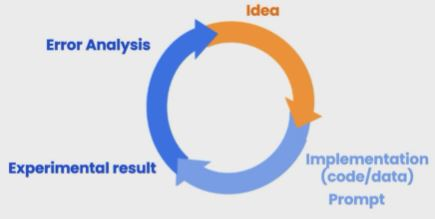
\includegraphics{images/iterative.jpg}

}

\end{figure}

\begin{itemize}
\tightlist
\item
  começamos com um \emph{prompt} claro e específico;
\item
  analisamos porque é que o resultado não dá o \emph{output} desejado;
\item
  afinamos a ideia e o \emph{prompt};
\item
  repetimos.
\end{itemize}

Gerar uma descrição de marketing a partir de uma ficha informativa do
produto.

\begin{Shaded}
\begin{Highlighting}[]
\NormalTok{ficha\_produto }\OtherTok{\textless{}{-}} \StringTok{"VISÃO GERAL}
\StringTok{{-} Parte de uma bela família de móveis de escritório inspirados em meados do século,}
\StringTok{incluindo armários de arquivo, escrivaninhas, estantes de livros, mesas de reunião e muito mais.}
\StringTok{{-} Diversas opções de cores de casca e acabamentos de base.}
\StringTok{{-} Disponível com estofamento traseiro e frontal de plástico (SWC{-}100)}
\StringTok{ou estofamento completo (SWC{-}110) em 10 opções de tecido e 6 opções de couro.}
\StringTok{{-} As opções de acabamento da base são: aço inoxidável, preto fosco,}
\StringTok{branco brilhante ou cromado.}
\StringTok{{-} A cadeira está disponível com ou sem braços.}
\StringTok{{-} Adequado para ambientes domésticos ou empresariais.}
\StringTok{{-} Qualificado para uso contratual.}

\StringTok{CONSTRUÇÃO}
\StringTok{{-} Base em alumínio revestido a plástico com 5 rodas.}
\StringTok{{-} Ajuste pneumático da cadeira para facilitar a ação de subir/baixar.}

\StringTok{DIMENSÕES}
\StringTok{{-} LARGURA 53 CM | 20,87”}
\StringTok{{-} PROFUNDIDADE 51 CM | 20,08”}
\StringTok{{-} ALTURA 80 CM | 31,50”}
\StringTok{{-} ALTURA DO ASSENTO 44 CM | 17,32”}
\StringTok{{-} PROFUNDIDADE DO ASSENTO 41 CM | 16,14”}

\StringTok{OPÇÕES}
\StringTok{{-} Opções de rodízios para piso macio ou duro.}
\StringTok{{-} Duas opções de densidades de espuma de assento:}
\StringTok{ médio (1,8 lb/ft3) ou alto (2,8 lb/ft3)}
\StringTok{{-} Apoios de braço em PU sem braços ou com 8 posições}

\StringTok{MATERIAIS}
\StringTok{PLANADOR DE BASE DE CONCHA}
\StringTok{{-} Alumínio fundido com revestimento de nylon modificado PA6/PA66.}
\StringTok{{-} Espessura da casca: 10 mm.}
\StringTok{ASSENTO}
\StringTok{{-} Espuma HD36}

\StringTok{PAÍS DE ORIGEM}
\StringTok{{-} Itália"}

\NormalTok{prompt0 }\OtherTok{\textless{}{-}} \FunctionTok{paste}\NormalTok{(}\StringTok{"A tua tarefa é ajudar a equipa de markting a criar a descrição }
\StringTok{para um website de vendas com base numa ficha de produto.}

\StringTok{Escreve a descrição do produto com base na informação fornecida }
\StringTok{nas especificações técnivas delimitadas por triplas plicas.}

\StringTok{Especificaações técnicas: \textquotesingle{}\textquotesingle{}\textquotesingle{} "}\NormalTok{, ficha\_produto, }\StringTok{"\textquotesingle{}\textquotesingle{}\textquotesingle{} "}\NormalTok{)}

\NormalTok{resposta }\OtherTok{\textless{}{-}} \FunctionTok{get\_completion}\NormalTok{(prompt0)}

\NormalTok{resposta}
\end{Highlighting}
\end{Shaded}

\hypertarget{problema-1-o-texto-uxe9-muito-longo}{%
\section{Problema 1: o texto é muito
longo}\label{problema-1-o-texto-uxe9-muito-longo}}

\begin{itemize}
\tightlist
\item
  limita o número de palavras /frases / caracteres
\end{itemize}

\begin{Shaded}
\begin{Highlighting}[]
\NormalTok{prompt1 }\OtherTok{\textless{}{-}} \FunctionTok{paste}\NormalTok{(}\StringTok{"A tua tarefa é ajudar a equipa de markting a criar a descrição }
\StringTok{para um website de vendas com base numa ficha de produto.}

\StringTok{Escreve a descrição do produto com base na informação fornecida }
\StringTok{nas especificações técnivas delimitadas por triplas plicas.}

\StringTok{Usa no máximo 50 palavras.}

\StringTok{Especificações técnicas: \textquotesingle{}\textquotesingle{}\textquotesingle{} "}\NormalTok{, ficha\_produto, }\StringTok{"\textquotesingle{}\textquotesingle{}\textquotesingle{} "}\NormalTok{)}

\NormalTok{resposta }\OtherTok{\textless{}{-}} \FunctionTok{get\_completion}\NormalTok{(prompt1)}

\NormalTok{resposta}
\end{Highlighting}
\end{Shaded}

\hypertarget{problema-2-o-texto-foca-os-detalhes-errados}{%
\section{Problema 2: o texto foca os detalhes
errados}\label{problema-2-o-texto-foca-os-detalhes-errados}}

\begin{itemize}
\tightlist
\item
  pedir para fiocar nos aspecvtos relevantes para a audiência
\end{itemize}

\begin{Shaded}
\begin{Highlighting}[]
\NormalTok{prompt2 }\OtherTok{\textless{}{-}} \FunctionTok{paste}\NormalTok{(}\StringTok{"A tua tarefa é ajudar a equipa de markting a criar a descrição }
\StringTok{para um website de vendas com base numa ficha de produto.}

\StringTok{Escreve a descrição do produto com base na informação fornecida }
\StringTok{nas especificações técnivas delimitadas por triplas plicas.}

\StringTok{A descrição tem como destinatário os revendedores de miobiliário pelo que deve ser técnica}
\StringTok{na sua natureza e focar os materiais que fazem o produto.}

\StringTok{Usa no máximo 50 palavras.}

\StringTok{Especificações técnicas: \textquotesingle{}\textquotesingle{}\textquotesingle{} "}\NormalTok{, ficha\_produto, }\StringTok{"\textquotesingle{}\textquotesingle{}\textquotesingle{} "}\NormalTok{)}

\NormalTok{resposta }\OtherTok{\textless{}{-}} \FunctionTok{get\_completion}\NormalTok{(prompt2)}

\NormalTok{resposta}
\end{Highlighting}
\end{Shaded}

Incluir identificação do produto

\begin{Shaded}
\begin{Highlighting}[]
\NormalTok{prompt3 }\OtherTok{\textless{}{-}} \FunctionTok{paste}\NormalTok{(}\StringTok{"A tua tarefa é ajudar a equipa de markting a criar a descrição }
\StringTok{para um website de vendas com base numa ficha de produto.}

\StringTok{Escreve a descrição do produto com base na informação fornecida }
\StringTok{nas especificações técnivas delimitadas por triplas plicas.}

\StringTok{A descrição tem como destinatário os revendedores de miobiliário pelo que deve ser técnica}
\StringTok{na sua natureza e focar os materiais que fazem o produto.}

\StringTok{No final da descrição, incluir o ID do produto da especificação técnica.}

\StringTok{Usa no máximo 50 palavras.}

\StringTok{Especificações técnicas: \textquotesingle{}\textquotesingle{}\textquotesingle{} "}\NormalTok{, ficha\_produto, }\StringTok{"\textquotesingle{}\textquotesingle{}\textquotesingle{} "}\NormalTok{)}

\NormalTok{resposta }\OtherTok{\textless{}{-}} \FunctionTok{get\_completion}\NormalTok{(prompt3)}

\NormalTok{resposta}
\end{Highlighting}
\end{Shaded}

\hypertarget{problema-3-a-descriuxe7uxe3o-precisa-duma-tabela-de-dimesuxf5es}{%
\section{Problema 3: a descrição precisa duma tabela de
dimesões}\label{problema-3-a-descriuxe7uxe3o-precisa-duma-tabela-de-dimesuxf5es}}

\begin{itemize}
\tightlist
\item
  pedir para extrair informação e organizá-la numa tabela.
\end{itemize}

\begin{Shaded}
\begin{Highlighting}[]
\NormalTok{prompt4 }\OtherTok{\textless{}{-}} \FunctionTok{paste}\NormalTok{(}\StringTok{"A tua tarefa é ajudar a equipa de markting a criar a descrição }
\StringTok{para um website de vendas com base numa ficha de produto.}

\StringTok{Escreve a descrição do produto com base na informação fornecida }
\StringTok{nas especificações técnivas delimitadas por triplas plicas.}

\StringTok{A descrição tem como destinatário os revendedores de miobiliário pelo que deve ser técnica}
\StringTok{na sua natureza e focar os materiais que fazem o produto.}

\StringTok{No final da descrição, incluir o ID do produto da especificação técnica.}

\StringTok{Usa no máximo 50 palavras.}

\StringTok{Depois da descrição, incluir uma tabela que dá as dimensões do produto. }
\StringTok{A tabela deve ter duas colunas. Na primeira coluna incluir o nome das dimensões.}
\StringTok{Na segunda coluna incluir as medidas apenas em centimetros.}

\StringTok{Dá à tabela o título \textquotesingle{}Dimensões do produto\textquotesingle{}.}

\StringTok{Formata tudocomo HTML para que possa ser usado num website.}
\StringTok{Coloca a descrição num elemento \textless{}div\textgreater{}.}

\StringTok{Especificações técnicas: \textquotesingle{}\textquotesingle{}\textquotesingle{} "}\NormalTok{, ficha\_produto, }\StringTok{"\textquotesingle{}\textquotesingle{}\textquotesingle{} "}\NormalTok{)}

\NormalTok{resposta }\OtherTok{\textless{}{-}} \FunctionTok{get\_completion}\NormalTok{(prompt4)}

\NormalTok{resposta}
\end{Highlighting}
\end{Shaded}

\bookmarksetup{startatroot}

\hypertarget{summarizing}{%
\chapter{Summarizing}\label{summarizing}}

Resumir texto focando tópicos específicos.

\begin{Shaded}
\begin{Highlighting}[]
\NormalTok{rev\_produto }\OtherTok{\textless{}{-}} \StringTok{"Comprei este panda de peluxe no aniversário da minha filha, }
\StringTok{ela adora{-}o e leva{-}o para todo lado e leva para todo lugar. }
\StringTok{É macio e muito fofo, o seu rosto tem um ar amigável. }
\StringTok{Ainda assim é um pouco pequeno para o preço que paguei. }
\StringTok{Eu acho que pode haver outras opções maiores para o mesmo preço. }
\StringTok{Chegou um dia antes do esperado, então eu mesmo pude brincar com ele antes de lho entregar."}
\end{Highlighting}
\end{Shaded}

Resume com um limite de palavras / frases / caracteres.

\begin{Shaded}
\begin{Highlighting}[]
\NormalTok{prompt0 }\OtherTok{\textless{}{-}} \FunctionTok{paste}\NormalTok{(}\StringTok{"A tua tarefa é gerar um resumo curto duma revisão de produto dum site de e{-}commerce.}
\StringTok{                 Resume a revisão do produto entre plicas triplas num máximo de 30 palavras.}
\StringTok{                 Revisão: \textquotesingle{}\textquotesingle{}\textquotesingle{} "}\NormalTok{, rev\_produto, }\StringTok{" \textquotesingle{}\textquotesingle{}\textquotesingle{} "}\NormalTok{)}

\NormalTok{resposta }\OtherTok{\textless{}{-}} \FunctionTok{get\_completion}\NormalTok{(prompt0)}

\NormalTok{resposta}
\end{Highlighting}
\end{Shaded}

Resume com foco no transporte e entrega.

\begin{Shaded}
\begin{Highlighting}[]
\NormalTok{prompt1 }\OtherTok{\textless{}{-}} \FunctionTok{paste}\NormalTok{(}\StringTok{"A tua tarefa é gerar um resumo curto duma revisão de produtodum site de e{-}commerce.}
\StringTok{                 Resume a revisão entre plicas triplas num máximo de 30 palavras, }
\StringTok{                 com o foco em qualquer mençao no transporte e entrega do produto.}
\StringTok{                 Revisão: \textquotesingle{}\textquotesingle{}\textquotesingle{} "}\NormalTok{, rev\_produto, }\StringTok{" \textquotesingle{}\textquotesingle{}\textquotesingle{} "}\NormalTok{)}

\NormalTok{resposta }\OtherTok{\textless{}{-}} \FunctionTok{get\_completion}\NormalTok{(prompt1)}

\NormalTok{resposta}
\end{Highlighting}
\end{Shaded}

Resume com foco no preço e valor

\begin{Shaded}
\begin{Highlighting}[]
\NormalTok{prompt2 }\OtherTok{\textless{}{-}} \FunctionTok{paste}\NormalTok{(}\StringTok{"A tua tarefa é gerar um resumo curto duma revisão de produtodum site de e{-}commerce.}
\StringTok{                 Resume a revisão entre plicas triplas num máximo de 30 palavras, }
\StringTok{                 com o foco em qualquer mençao ao preço e e valor percepcionado.}
\StringTok{                 Revisão: \textquotesingle{}\textquotesingle{}\textquotesingle{} "}\NormalTok{, rev\_produto, }\StringTok{" \textquotesingle{}\textquotesingle{}\textquotesingle{} "}\NormalTok{)}

\NormalTok{resposta }\OtherTok{\textless{}{-}} \FunctionTok{get\_completion}\NormalTok{(prompt2)}

\NormalTok{resposta}
\end{Highlighting}
\end{Shaded}

\begin{itemize}
\tightlist
\item
  o resumo inclui topicos que não estão relacionados copm o focos
  definido.
\end{itemize}

Vamos tentar `extrair' em vez de `resumir'

\begin{Shaded}
\begin{Highlighting}[]
\NormalTok{prompt3 }\OtherTok{\textless{}{-}} \FunctionTok{paste}\NormalTok{(}\StringTok{"A tua tarefa é extrair informação relevante duma revisão de produto dum site de e{-}commerce.}
\StringTok{                 Extrai, da revisão do produto entre plicas triplas que se segue, }
\StringTok{                 informação relevante. Máximo de 30 palavras.}
\StringTok{                 Revisão: \textquotesingle{}\textquotesingle{}\textquotesingle{} "}\NormalTok{, rev\_produto, }\StringTok{" \textquotesingle{}\textquotesingle{}\textquotesingle{} "}\NormalTok{)}

\NormalTok{resposta }\OtherTok{\textless{}{-}} \FunctionTok{get\_completion}\NormalTok{(prompt3)}

\NormalTok{resposta}
\end{Highlighting}
\end{Shaded}

Resumir multiplas revisões

\begin{Shaded}
\begin{Highlighting}[]
\NormalTok{rev1 }\OtherTok{\textless{}{-}}\NormalTok{ rev\_produto}

\CommentTok{\# revisão de um candeeiro}
\NormalTok{rev2 }\OtherTok{\textless{}{-}} \StringTok{"Precisava de uma luminária bonita para meu quarto, }
\StringTok{e essa tinha armazenamento adicional e um preço não muito alto. }
\StringTok{Recebi rápido {-} chegou em 2 dias. A corda para a lâmpada quebrou }
\StringTok{durante o transporte e a empresa felizmente enviei um novo. }
\StringTok{Chegou em poucos dias depois. Foi fácil de montar. Então eu tive uma parte faltando,}
\StringTok{entrei em contato com a assistência deles e eles muito rapidamente me deram a peça que faltava! }
\StringTok{Parece{-}me ser uma grande empresa que se preocupa com seus clientes e produtos."}

\CommentTok{\# revisão de uma escova de dentes electrica}
\NormalTok{rev3 }\OtherTok{\textless{}{-}} \StringTok{"Meu higienista dental recomendou uma escova de dentes elétrica, por isso que comprei esta. }
\StringTok{A duração da bateria parece ser bastante impressionante até agora. }
\StringTok{Após o carregamento inicial e deixando o carregador conectado durante a primeira semana para }
\StringTok{condicionar a bateria, desliguei o carregador e tenho usado para escovar duas vezes ao dia }
\StringTok{nas últimas 3 semanas, tudo com a mesma carga. }
\StringTok{Mas a cabeça da escova de dentes é muito pequena. Já vi escovas de dentes para bebês maiores que esta}
\StringTok{Eu gostaria que a cabeça fosse maior com diferentes cerdas de comprimento para ficarem melhor entre os dentes porque este não. No geral, se você conseguir este em torno de US $ 50, é um bom negócio. }
\StringTok{As cabeças de reposição são muito caras, mas você pode}
\StringTok{obter genéricos com preços mais razoáveis. }
\StringTok{Essa escova de dentes me faz sentir como se tivesse ido ao dentista diariamente. }
\StringTok{Meus dentes parecem brilhantes e limpos!"}

\CommentTok{\# revisão de triturador}
\NormalTok{rev4 }\OtherTok{\textless{}{-}} \StringTok{"Então, eles ainda tinham o sistema de 17 peças em venda por cerca de 49 dólares no mês de novembro, }
\StringTok{cerca de metade do preço, mas, por alguma razão (chamem{-}lhe manipulação de preços) }
\StringTok{por volta da segunda semana de dezembro, os preços subiram todos }
\StringTok{para um valor entre 70 e 89 dólares pelo mesmo }
\StringTok{sistema. E o sistema de 11 peças subiu cerca de 10 dólares ou }
\StringTok{portanto, no preço, também em relação ao preço de venda anterior de 29 dólares.}
\StringTok{Parece bem, mas se olharmos para a base, a parte}
\StringTok{onde a lâmina encaixa no sítio não parece tão boa}
\StringTok{como nas edições anteriores de há uns anos atrás, mas eu }
\StringTok{tenciono ser muito delicado com ela (por exemplo, eu esmago }
\StringTok{itens muito duros como feijão, gelo, arroz, etc. no  }
\StringTok{liquidificador primeiro e depois pulverizo{-}os no tamanho da porção que}
\StringTok{quero na liquidificadora e depois mudo para a lâmina de bater }
\StringTok{para obter uma farinha mais fina, e utilizar a lâmina de corte transversal }
\StringTok{primeiro quando faço batidos, depois uso a lâmina plana }
\StringTok{se precisar de uma farinha mais fina/menos polposa). Dica especial para fazer batidos, }
\StringTok{corte finamente e congele os frutos e }
\StringTok{legumes (se usar espinafres, amoleça ligeiramente os  }
\StringTok{espinafres e depois congelar até estarem prontos a usar {-} e se estiver a fazer }
\StringTok{sorvete, use um processador de alimentos de tamanho pequeno a médio)  }
\StringTok{se planeia usar dessa forma pode evitar adicionar tanto }
\StringTok{gelo, se for o caso {-} ao fazer o seu smoothie. }
\StringTok{Passado cerca de um ano, o motor começou a fazer um ruído estranho. }
\StringTok{Liguei para o serviço de apoio ao cliente, mas a garantia já tinha expirado, }
\StringTok{pelo que tive de comprar outro. Para sua informação: }
\StringTok{A qualidade geral deste tipo de produtos tem vindo a diminuir, pelo que }
\StringTok{eles estão a contar com o reconhecimento da marca e }
\StringTok{fidelidade do consumidor para manter as vendas. Recebi{-}o em cerca de}
\StringTok{dois dias."}

\NormalTok{revisoes }\OtherTok{\textless{}{-}} \FunctionTok{c}\NormalTok{(rev1, rev2, rev3, rev4)}
\end{Highlighting}
\end{Shaded}

Aplicar um \emph{loop}

\begin{Shaded}
\begin{Highlighting}[]
\ControlFlowTok{for}\NormalTok{ (i }\ControlFlowTok{in} \DecValTok{1}\SpecialCharTok{:}\FunctionTok{length}\NormalTok{(revisoes))\{}
\NormalTok{  prompt }\OtherTok{\textless{}{-}} \FunctionTok{paste}\NormalTok{(}\StringTok{"A tua tarefa é extrair informação relevante duma revisão de produto dum site de e{-}commerce }
\StringTok{  para o departamento de expedição.}
\StringTok{                 Extrai, da revisão do produto entre plicas triplas que se segue, }
\StringTok{                 informação relevante. Máximo de 20 palavras.}
\StringTok{                 Revisão: \textquotesingle{}\textquotesingle{}\textquotesingle{} "}\NormalTok{, revisoes[i], }\StringTok{" \textquotesingle{}\textquotesingle{}\textquotesingle{} "}\NormalTok{)}

\NormalTok{resposta }\OtherTok{\textless{}{-}} \FunctionTok{get\_completion}\NormalTok{(prompt)}

\FunctionTok{cat}\NormalTok{(i)}
\FunctionTok{print}\NormalTok{(resposta)}
\NormalTok{\} }
\end{Highlighting}
\end{Shaded}

\bookmarksetup{startatroot}

\hypertarget{inferring}{%
\chapter{Inferring}\label{inferring}}

Inferir sentimentos e tópicos a partir de revisão de produtos.

\begin{Shaded}
\begin{Highlighting}[]
\NormalTok{rev\_lamp }\OtherTok{\textless{}{-}} \StringTok{"Precisava de um candeeiro bonito para o meu quarto, e este tinha }
\StringTok{arrumação adicional e um preço não muito elevado. }
\StringTok{Recebi{-}o rapidamente.  O fio do nosso candeeiro partiu{-}se durante o trasnporte }
\StringTok{e a empresa enviou de bom grado um novo. Também chegou em poucos dias depois. }
\StringTok{Foi fácil de montar.  Faltava{-}me uma peça, por isso contactei o apoio }
\StringTok{e eles arranjaram{-}me muito rapidamente a peça que faltava! }
\StringTok{A Lumina parece{-}me ser uma grande empresa que se preocupa com os seus clientes e produtos!!"}
\end{Highlighting}
\end{Shaded}

\hypertarget{sentimento-positivo-negativo}{%
\section{Sentimento (positivo /
negativo)}\label{sentimento-positivo-negativo}}

\begin{Shaded}
\begin{Highlighting}[]
\NormalTok{prompt0 }\OtherTok{\textless{}{-}} \FunctionTok{paste}\NormalTok{(}\StringTok{"Qual o sentimento da seguite revisão de produto delimitada por plicas triplas?}
\StringTok{                 Dá a resposta numa unica palavra: positivo ou negativo.}
\StringTok{                 Revisão: \textquotesingle{}\textquotesingle{}\textquotesingle{} "}\NormalTok{, rev\_lamp, }\StringTok{"\textquotesingle{}\textquotesingle{}\textquotesingle{}"}\NormalTok{)}

\NormalTok{resposta }\OtherTok{\textless{}{-}} \FunctionTok{get\_completion}\NormalTok{(prompt0)}

\NormalTok{resposta}
\end{Highlighting}
\end{Shaded}

\hypertarget{identifica-tipos-de-emouxe7uxf5es}{%
\section{Identifica tipos de
emoções}\label{identifica-tipos-de-emouxe7uxf5es}}

\begin{Shaded}
\begin{Highlighting}[]
\NormalTok{prompt1 }\OtherTok{\textless{}{-}} \FunctionTok{paste}\NormalTok{(}\StringTok{"Identifica uma lista de emoções que o escritor da seguinte revisão expressou.}
\StringTok{Não incluas mais de 5 items na lista. Formata a tua resposta como uma lista de palavras separadas por virgulas.}
\StringTok{                 Revisão: \textquotesingle{}\textquotesingle{}\textquotesingle{} "}\NormalTok{, rev\_lamp, }\StringTok{"\textquotesingle{}\textquotesingle{}\textquotesingle{}"}\NormalTok{)}

\NormalTok{resposta }\OtherTok{\textless{}{-}} \FunctionTok{get\_completion}\NormalTok{(prompt1)}

\NormalTok{resposta}
\end{Highlighting}
\end{Shaded}

\hypertarget{identifica-raiva}{%
\section{Identifica raiva}\label{identifica-raiva}}

\begin{Shaded}
\begin{Highlighting}[]
\NormalTok{prompt2 }\OtherTok{\textless{}{-}} \FunctionTok{paste}\NormalTok{(}\StringTok{"O escritor da seguinte revisão está com raiva?. }
\StringTok{A  revisão está delimitada por plicas triplas. A tua resposta deve ser: sim ou não.}
\StringTok{                 Revisão: \textquotesingle{}\textquotesingle{}\textquotesingle{} "}\NormalTok{, rev\_lamp, }\StringTok{"\textquotesingle{}\textquotesingle{}\textquotesingle{}"}\NormalTok{)}

\NormalTok{resposta }\OtherTok{\textless{}{-}} \FunctionTok{get\_completion}\NormalTok{(prompt2)}

\NormalTok{resposta}
\end{Highlighting}
\end{Shaded}

\hypertarget{extrai-classificadores}{%
\section{Extrai classificadores}\label{extrai-classificadores}}

Extrai os nomes do produto e da companhia a partir das revisão.

\begin{Shaded}
\begin{Highlighting}[]
\NormalTok{prompt3 }\OtherTok{\textless{}{-}} \FunctionTok{paste}\NormalTok{(}\StringTok{"Identifica os seguintes items da revisão:}
\StringTok{{-} Produto comprado;}
\StringTok{{-} Empresa que o produziu. }
\StringTok{A  revisão está delimitada por plicas triplas. }
\StringTok{A tua resposta deve ser uma tabela markdown com as colunas: Produto e Empresa.}
\StringTok{Se a informação não existir usa o valor NA. A tua resposta deve ser o mais curta possível.}

\StringTok{                 Revisão: \textquotesingle{}\textquotesingle{}\textquotesingle{} "}\NormalTok{, rev\_lamp, }\StringTok{"\textquotesingle{}\textquotesingle{}\textquotesingle{}"}\NormalTok{)}

\NormalTok{resposta }\OtherTok{\textless{}{-}} \FunctionTok{get\_completion}\NormalTok{(prompt3)}

\NormalTok{resposta}
\end{Highlighting}
\end{Shaded}

\hypertarget{multi-task}{%
\section{Multi task}\label{multi-task}}

Fazer várias tarefas ao mesmo tempo

\begin{Shaded}
\begin{Highlighting}[]
\NormalTok{prompt4 }\OtherTok{\textless{}{-}} \FunctionTok{paste}\NormalTok{(}\StringTok{"Identifica os seguintes items da revisão:}
\StringTok{{-} Semtimento (positivo ou negativo);}
\StringTok{{-} O revisor está com raiva?}
\StringTok{{-} Produto comprado;}
\StringTok{{-} Empresa que o produziu. }
\StringTok{A  revisão está delimitada por plicas triplas. }
\StringTok{A tua resposta deve ser uma tabela markdown com as colunas: Sentimento, Raiva, Produto e Empresa.}
\StringTok{Se a informação não existir usa o valor \textquotesingle{}NA\textquotesingle{}. A tua resposta deve ser o mais curta possível.}
\StringTok{O valor para Raiva deve ser booleano.}

\StringTok{                 Revisão: \textquotesingle{}\textquotesingle{}\textquotesingle{} "}\NormalTok{, rev\_lamp, }\StringTok{"\textquotesingle{}\textquotesingle{}\textquotesingle{}"}\NormalTok{)}

\NormalTok{resposta }\OtherTok{\textless{}{-}} \FunctionTok{get\_completion}\NormalTok{(prompt4)}

\NormalTok{resposta}
\end{Highlighting}
\end{Shaded}

\hypertarget{inferir-tuxf3picos}{%
\section{Inferir tópicos}\label{inferir-tuxf3picos}}

\begin{Shaded}
\begin{Highlighting}[]
\NormalTok{estoria }\OtherTok{\textless{}{-}} \StringTok{"Num inquérito recente realizado pelo governo, }
\StringTok{os funcionários do sector público foram convidados a avaliar o seu nível de }
\StringTok{de satisfação com o departamento em que trabalham. }
\StringTok{Os resultados revelaram que a NASA era o departamento mais popular }
\StringTok{com um índice de satisfação de 95\%.}

\StringTok{Um funcionário da NASA, John Smith, comentou os resultados, }
\StringTok{afirmando: \textquotesingle{}Não me surpreende que a NASA tenha ficado em primeiro lugar. }
\StringTok{É um ótimo lugar para trabalhar, com pessoas fantásticas e }
\StringTok{e oportunidades incríveis. Tenho orgulho em fazer parte de }
\StringTok{uma organização tão inovadora.\textquotesingle{}}

\StringTok{Os resultados também foram bem recebidos pela equipa de gestão da NASA, }
\StringTok{com o Diretor Tom Johnson a declarar: \textquotesingle{}Estamos entusiasmados por }
\StringTok{ouvir que os nossos funcionários estão satisfeitos com o seu trabalho na NASA. }
\StringTok{Temos uma equipa talentosa e dedicada que trabalha incansavelmente }
\StringTok{para atingir os nossos objectivos, e é fantástico ver que o seu }
\StringTok{trabalho árduo está a dar frutos\textquotesingle{}.}

\StringTok{O inquérito revelou também que a }
\StringTok{Administração da Segurança Social registou o índice de satisfação mais baixo }
\StringTok{com apenas 45\% dos empregados indicando que estavam }
\StringTok{satisfeitos com o seu trabalho. O Governo comprometeu{-}se a }
\StringTok{abordar as preocupações levantadas pelos funcionários no inquérito e }
\StringTok{trabalhar no sentido de melhorar a satisfação profissional em todos os departamentos.}
\StringTok{"}
\end{Highlighting}
\end{Shaded}

inferir 5 tópicos

\begin{Shaded}
\begin{Highlighting}[]
\NormalTok{prompt5 }\OtherTok{\textless{}{-}} \FunctionTok{paste}\NormalTok{(}\StringTok{"Determina 5 tópicos que estão a ser discutidos no texto seguinte }
\StringTok{que está delimitado por plicas triplas.}
\StringTok{Cada tópico deve ter apenas uma ou duas palavras.}
\StringTok{Formata a tua resposta numa lista de tópicos separados por virgulas.}

\StringTok{                 Texto: \textquotesingle{}\textquotesingle{}\textquotesingle{} "}\NormalTok{, estoria, }\StringTok{"\textquotesingle{}\textquotesingle{}\textquotesingle{}"}\NormalTok{)}

\NormalTok{resposta }\OtherTok{\textless{}{-}} \FunctionTok{get\_completion}\NormalTok{(prompt5)}

\NormalTok{resposta}
\end{Highlighting}
\end{Shaded}

\hypertarget{alertas}{%
\section{Alertas}\label{alertas}}

Fazer alertas para determinados tópicos

\begin{Shaded}
\begin{Highlighting}[]
\NormalTok{topicos }\OtherTok{\textless{}{-}} \FunctionTok{unlist}\NormalTok{(}\FunctionTok{strsplit}\NormalTok{(resposta,}\StringTok{","}\NormalTok{)) }\SpecialCharTok{|\textgreater{}} \FunctionTok{trimws}\NormalTok{()}

\ControlFlowTok{if}\NormalTok{( }\StringTok{\textquotesingle{}NASA\textquotesingle{}} \SpecialCharTok{\%in\%}\NormalTok{ topicos) }\FunctionTok{print}\NormalTok{(}\StringTok{\textquotesingle{}ALERT: notícias da NASA!\textquotesingle{}}\NormalTok{)}
\end{Highlighting}
\end{Shaded}

\bookmarksetup{startatroot}

\hypertarget{transforming}{%
\chapter{Transforming}\label{transforming}}

Um LLM pode também ser usado para em tarefas de transformação de texto,
como sejam a tradução, correcção gramatical, ajustar o tom e converter
formatos.

\hypertarget{traduuxe7uxe3o}{%
\section{Tradução}\label{traduuxe7uxe3o}}

O chatGPT está treinado com fontes de muitas línguas diferentes. Isto
permite ao modelo fazer traduções.

\begin{Shaded}
\begin{Highlighting}[]
\NormalTok{prompt0 }\OtherTok{\textless{}{-}} \StringTok{"Traduz o seguinte texto para italiano: \textquotesingle{}\textquotesingle{}\textquotesingle{} Olá, eu gostava de comprar um triturador. \textquotesingle{}\textquotesingle{}\textquotesingle{}"}

\NormalTok{resposta }\OtherTok{\textless{}{-}} \FunctionTok{get\_completion}\NormalTok{(prompt0)}

\NormalTok{resposta}
\end{Highlighting}
\end{Shaded}

\begin{Shaded}
\begin{Highlighting}[]
\NormalTok{prompt1 }\OtherTok{\textless{}{-}} \StringTok{"Diz{-}me em que linguagem está isto: \textquotesingle{}Combien coûte le lampadaire?\textquotesingle{} "}

\NormalTok{resposta }\OtherTok{\textless{}{-}} \FunctionTok{get\_completion}\NormalTok{(prompt1)}

\NormalTok{resposta}
\end{Highlighting}
\end{Shaded}

\begin{Shaded}
\begin{Highlighting}[]
\NormalTok{prompt2 }\OtherTok{\textless{}{-}} \StringTok{"Traduz o seguinte texto para espanhol e }
\StringTok{italiano e ingles de pirata: \textquotesingle{}\textquotesingle{}\textquotesingle{}Quero encomendar uma bola de basketball.\textquotesingle{}\textquotesingle{}\textquotesingle{} "}

\NormalTok{resposta }\OtherTok{\textless{}{-}} \FunctionTok{get\_completion}\NormalTok{(prompt2)}

\NormalTok{resposta}
\end{Highlighting}
\end{Shaded}

Tradução de múltiplas frases em diferentes línguas.

\begin{Shaded}
\begin{Highlighting}[]
\NormalTok{mensagens }\OtherTok{\textless{}{-}} \FunctionTok{c}\NormalTok{(}\StringTok{"La performance du système est plus lente que d\textquotesingle{}habitude."}\NormalTok{,  }
               \StringTok{"Mi monitor tiene píxeles que no se iluminan."}\NormalTok{,}
               \StringTok{"Il mio mouse non funziona"}\NormalTok{,}
               \StringTok{"Mój klawisz Ctrl jest zepsuty"}\NormalTok{,}
               \StringTok{"我的屏幕在闪烁"}\NormalTok{)}

\ControlFlowTok{for}\NormalTok{ (i }\ControlFlowTok{in} \DecValTok{1}\SpecialCharTok{:} \FunctionTok{length}\NormalTok{(mensagens))\{}
\NormalTok{  prompt3 }\OtherTok{\textless{}{-}} \FunctionTok{paste}\NormalTok{(}\StringTok{"Numa só palavra, diz{-}me em que lingua está a frase:"}\NormalTok{, mensagens[i])}
\NormalTok{  lingua }\OtherTok{\textless{}{-}} \FunctionTok{get\_completion}\NormalTok{(prompt3)}
\NormalTok{  resposta }\OtherTok{\textless{}{-}} \FunctionTok{get\_completion}\NormalTok{(}\FunctionTok{paste}\NormalTok{(}\StringTok{"traduz para português:"}\NormalTok{, mensagens[i]))}
  
  \FunctionTok{print}\NormalTok{(}\FunctionTok{paste}\NormalTok{(}\StringTok{"A língua original é:"}\NormalTok{, lingua,}\StringTok{".}\SpecialCharTok{\textbackslash{}n}\StringTok{"}\NormalTok{,}
              \StringTok{"A tradução é:"}\NormalTok{, resposta))}
  
\NormalTok{\}}
\end{Highlighting}
\end{Shaded}

\hypertarget{modificauxe7uxe3o-do-tom}{%
\section{Modificação do tom}\label{modificauxe7uxe3o-do-tom}}

De acordo com a nossa audiência podemos definir o nosso tom.

\begin{Shaded}
\begin{Highlighting}[]
\NormalTok{frase }\OtherTok{\textless{}{-}} \StringTok{"Mano, este é o Zé, tipo vê só as cenas desta lamparina!"} 

\NormalTok{prompt4 }\OtherTok{\textless{}{-}} \FunctionTok{paste}\NormalTok{(}\StringTok{"Traduz a frase do calão para uma linguagem formal de negócio:"}\NormalTok{, frase)}

\NormalTok{resposta }\OtherTok{\textless{}{-}} \FunctionTok{get\_completion}\NormalTok{(prompt4)}

\NormalTok{resposta}
\end{Highlighting}
\end{Shaded}

\hypertarget{conversuxe3o-de-formato}{%
\section{Conversão de formato}\label{conversuxe3o-de-formato}}

\begin{Shaded}
\begin{Highlighting}[]
\NormalTok{df }\OtherTok{\textless{}{-}} \FunctionTok{data.frame}\NormalTok{(}\AttributeTok{nome =} \FunctionTok{c}\NormalTok{(}\StringTok{\textquotesingle{}Sérgio\textquotesingle{}}\NormalTok{,}\StringTok{\textquotesingle{}Bruno\textquotesingle{}}\NormalTok{,}\StringTok{\textquotesingle{}José\textquotesingle{}}\NormalTok{),}
                 \AttributeTok{email =} \FunctionTok{c}\NormalTok{(}\StringTok{\textquotesingle{}sergio.cenas@gmail.com\textquotesingle{}}\NormalTok{,}\StringTok{\textquotesingle{}b2578@gmail.com\textquotesingle{}}\NormalTok{,}\StringTok{\textquotesingle{}zedecima@gmail.com\textquotesingle{}}\NormalTok{))}

\NormalTok{prompt5 }\OtherTok{\textless{}{-}} \FunctionTok{paste}\NormalTok{(}\StringTok{"Traduz o data.frame para uma tabela HTML:"}\NormalTok{, }
\NormalTok{                df)}
\NormalTok{resposta }\OtherTok{\textless{}{-}} \FunctionTok{get\_completion}\NormalTok{(prompt5)}

\NormalTok{resposta}
\end{Highlighting}
\end{Shaded}

\hypertarget{correcuxe7auxf5-ortogruxe1fica}{%
\section{Correcçaõ ortográfica}\label{correcuxe7auxf5-ortogruxe1fica}}

\begin{Shaded}
\begin{Highlighting}[]
\NormalTok{frases }\OtherTok{\textless{}{-}} \FunctionTok{c}\NormalTok{(}\StringTok{\textquotesingle{}A rapariga com os caes brancos e pretos ter uma bola.\textquotesingle{}}\NormalTok{,}
            \StringTok{\textquotesingle{}A Yolanda tem o seu caderno.\textquotesingle{}}\NormalTok{,}
            \StringTok{\textquotesingle{}Foi ser um dia longo. À peixe para jantar.\textquotesingle{}}\NormalTok{,}
            \StringTok{\textquotesingle{}Esta tem erros gramalticais.\textquotesingle{}}\NormalTok{,}
            \StringTok{\textquotesingle{}Descancar é muito mais melhor bom.\textquotesingle{}}
\NormalTok{            )}

\ControlFlowTok{for}\NormalTok{(i }\ControlFlowTok{in} \DecValTok{1}\SpecialCharTok{:}\FunctionTok{length}\NormalTok{(frases))\{}
\NormalTok{  prompt6 }\OtherTok{\textless{}{-}} \FunctionTok{paste}\NormalTok{(}\StringTok{"Corrige a frase entre plicas triplas e reescreve{-}a de forma correcta. }
\StringTok{                 Se não houver nenhum erro apenas devolve: \textquotesingle{}Não encontrei erros!\textquotesingle{}: \textquotesingle{}\textquotesingle{}\textquotesingle{}"}\NormalTok{, frases[i], }\StringTok{"\textquotesingle{}\textquotesingle{}\textquotesingle{}"}\NormalTok{)}
\NormalTok{  resposta }\OtherTok{\textless{}{-}} \FunctionTok{get\_completion}\NormalTok{(prompt6)}
  \FunctionTok{print}\NormalTok{(}\FunctionTok{paste}\NormalTok{(}\StringTok{"Frase"}\NormalTok{, i, }\StringTok{":"}\NormalTok{, resposta))}
\NormalTok{\}}
\end{Highlighting}
\end{Shaded}

\begin{Shaded}
\begin{Highlighting}[]
\NormalTok{texto }\OtherTok{\textless{}{-}} \StringTok{"Comprei isto para a minha filha no seu aniversário, porque ela está sempre a tirar}
\StringTok{os meus do meu quarto.  Sim, os adultos também gostam de pandas.  Ela leva{-}o}
\StringTok{para todo o lado com ela, porque é super macio e giro.  Uma das orelhas  }
\StringTok{é um pouco mais pequena do que a outra, e acho que não foi feito para ser assimétrico. }
\StringTok{É um pouco pequeno para o que paguei por ele. No entanto, penso que pode haver outras opções que sejam maiores pelo o mesmo preço.  Chegou um dia antes do previsto, por isso pude brincar com ele antes de o dar à minha filha."}

\NormalTok{prompt7 }\OtherTok{\textless{}{-}} \FunctionTok{paste}\NormalTok{(}\StringTok{"Reve e corrige a revisão que está entre plicas triplas. Torna{-}a mais convincente.}
\StringTok{                 Assegura que segue o guia de estilo APA e que se destina a um leitor avançado. }
\StringTok{                 O output deve estar em formato markdown: \textquotesingle{}\textquotesingle{}\textquotesingle{} "}\NormalTok{, texto, }\StringTok{"\textquotesingle{}\textquotesingle{}\textquotesingle{}"}\NormalTok{)}

\NormalTok{resposta }\OtherTok{\textless{}{-}} \FunctionTok{get\_completion}\NormalTok{(prompt7)}

\NormalTok{resposta}
\end{Highlighting}
\end{Shaded}

\bookmarksetup{startatroot}

\hypertarget{expanding}{%
\chapter{Expanding}\label{expanding}}

Vamos gerar respostas automáticas

\begin{Shaded}
\begin{Highlighting}[]
\NormalTok{sente }\OtherTok{\textless{}{-}} \StringTok{\textquotesingle{}negativo\textquotesingle{}}

\NormalTok{revisao }\OtherTok{\textless{}{-}} \StringTok{"Afinal, eles ainda tinham o sistema de 17 peças à }
\StringTok{venda por cerca de 49 dólares no mês de novembro, cerca de metade do preço, }
\StringTok{mas, por alguma razão (chamem{-}lhe manipulação de preços) por volta da segunda semana de dezembro, }
\StringTok{os preços subiram todos para um valor entre 70 e 89 dólares pelo mesmo sistema. }
\StringTok{E o sistema de 11 peças subiu cerca de 10 dólares, também em relação ao preço de venda anterior de 29 dólares.}
\StringTok{Parece bem, mas se olharmos para a base, a parte onde a lâmina encaixa no sítio não parece tão boa}
\StringTok{como nas edições anteriores de há uns anos atrás, mas eu tenciono ser muito delicado com ela }
\StringTok{(por exemplo, eu esmago itens muito duros como feijão, gelo, arroz, etc. no liquidificador primeiro e depois pulverizo{-}os no tamanho da porção que quero na liquidificadora }
\StringTok{e depois mudo para a lâmina de bater para obter uma farinha mais fina, }
\StringTok{e utilizo a lâmina de corte transversal primeiro quando faço batidos, }
\StringTok{depois uso a lâmina plana se precisar de uma farinha mais fina/menos polposa). }
\StringTok{Dica especial para fazer batidos, corte finamente e congele os frutos e legumes }
\StringTok{(se usar espinafres, amoleça ligeiramente os espinafres e depois congelar até estarem prontos a usar }
\StringTok{{-} e se estiver a fazer sorvete, use um processador de alimentos de tamanho pequeno a médio) }
\StringTok{dessa forma pode evitar adicionar muito gelo, ao fazer o seu smoothie. }
\StringTok{Passado cerca de um ano, o motor começou a fazer um ruído estranho. }
\StringTok{Liguei para o serviço de apoio ao cliente, mas a garantia já tinha expirado, }
\StringTok{pelo que tive de comprar outro. Para sua informação: }
\StringTok{A qualidade geral deste tipo de produtos tem vindo a diminuir, pelo que }
\StringTok{eles estão a contar com o reconhecimento da marca e }
\StringTok{fidelidade do consumidor para manter as vendas. }
\StringTok{Recebi{-}o em cerca de dois dias."} 

\NormalTok{prompt0 }\OtherTok{\textless{}{-}} \FunctionTok{paste}\NormalTok{(}\StringTok{"Tu és um assistente AI de serviço ao cliente. A tua tarefa é mandar um e{-}mail de resposta}
\StringTok{                 para um importante cliente. O email do cliente está delimitado por plicas triplas.}
\StringTok{                 Se o \textless{} sentimento \textgreater{} for positivo ou neutro, agradece o comentário. Se o sentimento for negativo,}
\StringTok{                 pede desculpa e sugere que podem contar com o serviço ao cliente.}
\StringTok{                 Garante que fazes referencia a especificidade do comentário. }
\StringTok{                 Escreve o email num tom profissional e sintético.}
\StringTok{                 Assina o e{-}mail como \textasciigrave{}Agente AI ao cliente\textasciigrave{}. Comentário do cliente: \textquotesingle{}\textquotesingle{}\textquotesingle{}"}\NormalTok{,}
\NormalTok{                 revisao, }\StringTok{" \textquotesingle{}\textquotesingle{}\textquotesingle{}; Sentimento do comentário: \textless{}"}\NormalTok{, sente, }\StringTok{"\textgreater{}"}\NormalTok{)}

\NormalTok{resposta }\OtherTok{\textless{}{-}} \FunctionTok{get\_completion}\NormalTok{(prompt0)}

\NormalTok{resposta}
\end{Highlighting}
\end{Shaded}

\bookmarksetup{startatroot}

\hypertarget{chatbot}{%
\chapter{Chatbot}\label{chatbot}}

Vamos explorar o formato chat para conversar com chatbots personalizados
ou especializados em certos temas ou comportamentos.

A função \texttt{create\_chat\_completion} do \emph{package} \{openai\}
permite ter este tipo de diálogos.

\begin{Shaded}
\begin{Highlighting}[]
\NormalTok{res }\OtherTok{\textless{}{-}} \FunctionTok{create\_chat\_completion}\NormalTok{(}
   \AttributeTok{model =} \StringTok{"gpt{-}3.5{-}turbo"}\NormalTok{,}
   \AttributeTok{messages =} \FunctionTok{list}\NormalTok{(}
       \FunctionTok{list}\NormalTok{(}
           \StringTok{"role"} \OtherTok{=} \StringTok{"system"}\NormalTok{,}
           \StringTok{"content"} \OtherTok{=} \StringTok{"És um assistente que fala como o Camões"}
\NormalTok{       ),}
       \FunctionTok{list}\NormalTok{(}
           \StringTok{"role"} \OtherTok{=} \StringTok{"user"}\NormalTok{,}
           \StringTok{"content"} \OtherTok{=} \StringTok{"Conta{-}me uma anedota."}
\NormalTok{       ),}
       \FunctionTok{list}\NormalTok{(}
           \StringTok{"role"} \OtherTok{=} \StringTok{"assistant"}\NormalTok{,}
           \StringTok{"content"} \OtherTok{=} \StringTok{"Porque é que a galinha atravessou a estrada?"}
\NormalTok{       ),}
       \FunctionTok{list}\NormalTok{(}
           \StringTok{"role"} \OtherTok{=} \StringTok{"user"}\NormalTok{,}
           \StringTok{"content"} \OtherTok{=} \StringTok{"Não sei."}
\NormalTok{       )}
\NormalTok{   )}
\NormalTok{)}

\NormalTok{res}\SpecialCharTok{$}\NormalTok{choices}\SpecialCharTok{$}\NormalTok{message.content}
\end{Highlighting}
\end{Shaded}

\begin{Shaded}
\begin{Highlighting}[]
\NormalTok{res }\OtherTok{\textless{}{-}} \FunctionTok{create\_chat\_completion}\NormalTok{(}
   \AttributeTok{model =} \StringTok{"gpt{-}3.5{-}turbo"}\NormalTok{,}
   \AttributeTok{messages =} \FunctionTok{list}\NormalTok{(}
       \FunctionTok{list}\NormalTok{(}
           \StringTok{"role"} \OtherTok{=} \StringTok{"system"}\NormalTok{,}
           \StringTok{"content"} \OtherTok{=} \StringTok{"És um chatbot amistoso"}
\NormalTok{       ),}
       \FunctionTok{list}\NormalTok{(}
           \StringTok{"role"} \OtherTok{=} \StringTok{"user"}\NormalTok{,}
           \StringTok{"content"} \OtherTok{=} \StringTok{"Olá, chamo{-}me Elsa."}
\NormalTok{       )}
\NormalTok{       )}
\NormalTok{   )}

\NormalTok{res}\SpecialCharTok{$}\NormalTok{choices}\SpecialCharTok{$}\NormalTok{message.content}

\FunctionTok{create\_chat\_completion}\NormalTok{(}
   \AttributeTok{model =} \StringTok{"gpt{-}3.5{-}turbo"}\NormalTok{,}
   \AttributeTok{messages =} \FunctionTok{list}\NormalTok{(}
       \FunctionTok{list}\NormalTok{(}
           \StringTok{"role"} \OtherTok{=} \StringTok{"system"}\NormalTok{,}
           \StringTok{"content"} \OtherTok{=} \StringTok{"És um chatbot amistoso"}
\NormalTok{       ),}
       \FunctionTok{list}\NormalTok{(}
           \StringTok{"role"} \OtherTok{=} \StringTok{"user"}\NormalTok{,}
           \StringTok{"content"} \OtherTok{=} \StringTok{"Podes lembrar{-}me como me chamo?"}
\NormalTok{       )}
\NormalTok{       )}
\NormalTok{   )}\SpecialCharTok{$}\NormalTok{choices}\SpecialCharTok{$}\NormalTok{message.content}
\end{Highlighting}
\end{Shaded}

O chatbot não sabe o nome pois cada conversa está delimitada por
execução da função, ou seja, cada conversa é uma interacção
\emph{standalone}.

\begin{Shaded}
\begin{Highlighting}[]
\NormalTok{res }\OtherTok{\textless{}{-}} \FunctionTok{create\_chat\_completion}\NormalTok{(}
   \AttributeTok{model =} \StringTok{"gpt{-}3.5{-}turbo"}\NormalTok{,}
   \AttributeTok{messages =} \FunctionTok{list}\NormalTok{(}
       \FunctionTok{list}\NormalTok{(}
           \StringTok{"role"} \OtherTok{=} \StringTok{"system"}\NormalTok{,}
           \StringTok{"content"} \OtherTok{=} \StringTok{"És um chatbot amistoso"}
\NormalTok{       ),}
       \FunctionTok{list}\NormalTok{(}
           \StringTok{"role"} \OtherTok{=} \StringTok{"user"}\NormalTok{,}
           \StringTok{"content"} \OtherTok{=} \StringTok{"Olá, chamo{-}me Bruno."}
\NormalTok{       ),}
       \FunctionTok{list}\NormalTok{(}
           \StringTok{"role"} \OtherTok{=} \StringTok{"assistant"}\NormalTok{,}
           \StringTok{"content"} \OtherTok{=} \StringTok{"Olá Bruno, em que te posso ajudar?"}
\NormalTok{       ),}
       \FunctionTok{list}\NormalTok{(}
           \StringTok{"role"} \OtherTok{=} \StringTok{"user"}\NormalTok{,}
           \StringTok{"content"} \OtherTok{=} \StringTok{"Podes lembrar{-}me como me chamo?"}
\NormalTok{       )}
\NormalTok{   )}
\NormalTok{)}

\NormalTok{res}\SpecialCharTok{$}\NormalTok{choices}\SpecialCharTok{$}\NormalTok{message.content}
\end{Highlighting}
\end{Shaded}

Agora o modelo já sabe responder.

\begin{Shaded}
\begin{Highlighting}[]
\NormalTok{instrucao }\OtherTok{\textless{}{-}} \StringTok{"Tu és o OrderBot, um serviço automatizado que regista os pedidos e }
\StringTok{           depois pergunta onde é a entrega. Recebes o pedido inteiro depois fazes }
\StringTok{           o seu resumo e dizes qual é o preço. O menu inclui: pizza peperoni: 10€;}
\StringTok{           pizza de queijo: 9€;}
\StringTok{           pizza vegetariana: 15€;}
\StringTok{           batatas: 5€}
\StringTok{           salada: 4€}
\StringTok{           molho: 2€}
\StringTok{           bebida: 7€"}

\NormalTok{res }\OtherTok{\textless{}{-}} \FunctionTok{create\_chat\_completion}\NormalTok{(}
   \AttributeTok{model =} \StringTok{"gpt{-}3.5{-}turbo"}\NormalTok{,}
   \AttributeTok{messages =} \FunctionTok{list}\NormalTok{(}
       \FunctionTok{list}\NormalTok{(}
           \StringTok{"role"} \OtherTok{=} \StringTok{"system"}\NormalTok{,}
           \StringTok{"content"} \OtherTok{=}\NormalTok{ instrucao}
\NormalTok{       ),}
       \FunctionTok{list}\NormalTok{(}
           \StringTok{"role"} \OtherTok{=} \StringTok{"user"}\NormalTok{,}
           \StringTok{"content"} \OtherTok{=} \StringTok{"Olá, chamo{-}me Bruno."}
\NormalTok{       ),}
       \FunctionTok{list}\NormalTok{(}
           \StringTok{"role"} \OtherTok{=} \StringTok{"assistant"}\NormalTok{,}
           \StringTok{"content"} \OtherTok{=} \StringTok{"Olá Bruno, qual é o teu pedido?"}
\NormalTok{       ),}
       \FunctionTok{list}\NormalTok{(}
           \StringTok{"role"} \OtherTok{=} \StringTok{"user"}\NormalTok{,}
           \StringTok{"content"} \OtherTok{=} \FunctionTok{readline}\NormalTok{()}
\NormalTok{       )}
\NormalTok{   )}
\NormalTok{)}

\NormalTok{res}\SpecialCharTok{$}\NormalTok{choices}\SpecialCharTok{$}\NormalTok{message.content}
\end{Highlighting}
\end{Shaded}

Podemos usar o package \href{https://openair-lib.org/}{\{OpenAIR\}} para
termos um chatbot à nossa medida e com o qual possamos interatuar.

\begin{Shaded}
\begin{Highlighting}[]
\FunctionTok{library}\NormalTok{(devtools)}
\NormalTok{devtools}\SpecialCharTok{::}\FunctionTok{install\_github}\NormalTok{(}\StringTok{"umatter/OpenAIR"}\NormalTok{)}

\FunctionTok{library}\NormalTok{(}\StringTok{"TheOpenAIR"}\NormalTok{)}

\FunctionTok{chat}\NormalTok{(instrucao)}

\FunctionTok{chat}\NormalTok{(}\StringTok{"eu não fiz esse pedido. Quero fazer um pedido novo"}\NormalTok{)}

\FunctionTok{chat}\NormalTok{(}\StringTok{"quero uma pizza de queijo com salada, molho e duas bebidas"}\NormalTok{)}
\end{Highlighting}
\end{Shaded}

Este package permitemos fazer coisas tão simples como \emph{RegExp}
através de comandos escritos

\begin{Shaded}
\begin{Highlighting}[]
\NormalTok{resp }\OtherTok{\textless{}{-}} \StringTok{"Remove todos os numeros de \textquotesingle{}5XC{-}2a09ujnap9o2q0MP\textquotesingle{}}
\StringTok{a tua resposta deverá ter apenas os caracteres que sobram"} \SpecialCharTok{\%c\%}
  \StringTok{"message"} 

\NormalTok{resp}
\end{Highlighting}
\end{Shaded}

\bookmarksetup{startatroot}

\hypertarget{conclusion}{%
\chapter{Conclusion}\label{conclusion}}

A utilização do \emph{chatGPT} em modo de desenvolvimento com o R
permite explorar novos horizontes.

A apreenção destes conceitos mais básicos que aqui foram apresentados, é
um ponto de partida para uma utilização mais exaustiva desta nova
ferramenta.

São já muitos os \emph{packages} relacionados que podemos encontrar no
CRAN:

\begin{longtable}[]{@{}
  >{\raggedright\arraybackslash}p{(\columnwidth - 2\tabcolsep) * \real{0.5000}}
  >{\raggedright\arraybackslash}p{(\columnwidth - 2\tabcolsep) * \real{0.5000}}@{}}
\toprule\noalign{}
\begin{minipage}[b]{\linewidth}\raggedright
\emph{package}
\end{minipage} & \begin{minipage}[b]{\linewidth}\raggedright
descrição
\end{minipage} \\
\midrule\noalign{}
\endhead
\bottomrule\noalign{}
\endlastfoot
\href{https://cran.r-project.org/web/packages/chatAI4R/index.html}{chatAI4R}
& Chat-Based Interactive Artificial Intelligence for R \\
\href{https://cran.r-project.org/web/packages/chatgpt/index.html}{chatgpt}
& Interface to `ChatGPT' from R \\
\href{https://cran.r-project.org/web/packages/openai/}{openai} & R
Wrapper for OpenAI API \\
\end{longtable}

ou outros disponíveis através do github:

\begin{longtable}[]{@{}
  >{\raggedright\arraybackslash}p{(\columnwidth - 2\tabcolsep) * \real{0.5000}}
  >{\raggedright\arraybackslash}p{(\columnwidth - 2\tabcolsep) * \real{0.5000}}@{}}
\toprule\noalign{}
\begin{minipage}[b]{\linewidth}\raggedright
\emph{package}
\end{minipage} & \begin{minipage}[b]{\linewidth}\raggedright
descrição
\end{minipage} \\
\midrule\noalign{}
\endhead
\bottomrule\noalign{}
\endlastfoot
\href{https://openair-lib.org/}{TheOpenAIR} & Integrate `OpenAI' Large
Language Models into Your `R' Workflows \\
\href{https://mlverse.github.io/chattr/}{chattr} & It enables
interaction with LLM directly from the RStudio IDE \\
\end{longtable}

Certamente que estas listas irão aumentar à medida das necessidades dos
utilizadores de R.

\bookmarksetup{startatroot}

\hypertarget{references}{%
\chapter{References}\label{references}}


\backmatter

\end{document}
